In this section we go over the three workflows that the pipeline offers, see figures \ref{fig:pipelineRun}. We have a normal integration workflow, a multimodal integration workflow if the dataset also contains additional data like protein data and a workflow for HTO demultiplexing. All three mostly follow the guidelines described in Seurat's vignettes. In general, all workflows work similarly. 

Start by filling out the minimal inputs needed in your config.yaml. More on this in section~\ref{section:config}. Next, run the pipeline with a command. For how to run the pipeline please see section~\ref{section:runPipeline}. If this is the first time using the pipeline, the pipeline should start by creating certain conda environments where some dependencies need to be installed manually via a script, see figure~\ref{fig:installRun}. After the installation, we can begin with the actual analysis. 

Use the pipeline command again. The pipeline should start running again. After a while the pipeline will throw an \textbf{\textit{MissingInputError}} exception. This is a custom exception made for the pipeline and completely normal. The exception is thrown when the pipeline needs an input that the user might not know at the very beginning. After the user entered the input into the config.yaml, the pipeline run can continue by using the run command again.\\

E.g.: After the rule \textit{mt\_p1} is finished it will have created a plot named sample\_name.mt.before.pdf for each sample in the dataset. If a single \textit{mtCutoff} of a sample is not filled out in the config.yaml the pipeline will throw a \textbf{\textit{MissingInputError}} exception. The exception will either print a message in the terminal or write the error message into the clusterLogs/ or logs/ file depending on how the pipeline is run. In this case the message will ask the user to take a look at each sample\_name.mt.before.pdf to decide at what percentage the mitochondrial reads should be filtered and ask the user to fill out the respective entry in the config.yaml before starting the pipeline again.\\

If the user does not want these interruptions and \textbf{instead prefers a single uninterrupted run}, they can fill in the missing entries in the config.yaml at the very beginning if they are confident that they know the values without looking at plots.\\

All points where interruptions can occur and which entry would be missing is also shown in figure~\ref{fig:pipelineRun} at the dashed/dotted arrows along with the stop sign nodes.\\

In the following subsections we will briefly go over each of the pipeline steps. Bold words will be placeholders.

\subsection{installMissingPackages}
The steps createDoubletEnv, createShinyEnv and createCountEnv create conda environments for installMissingPackages which will install the dependencies from the dependencies/ folder into these environments, see figure~\ref{fig:installRun}.

\begin{figure}[h!]
	%\includesvg[width=\textwidth]{figures/pipelineRun.pdf}
	\centering
	\makebox[\textwidth][c]{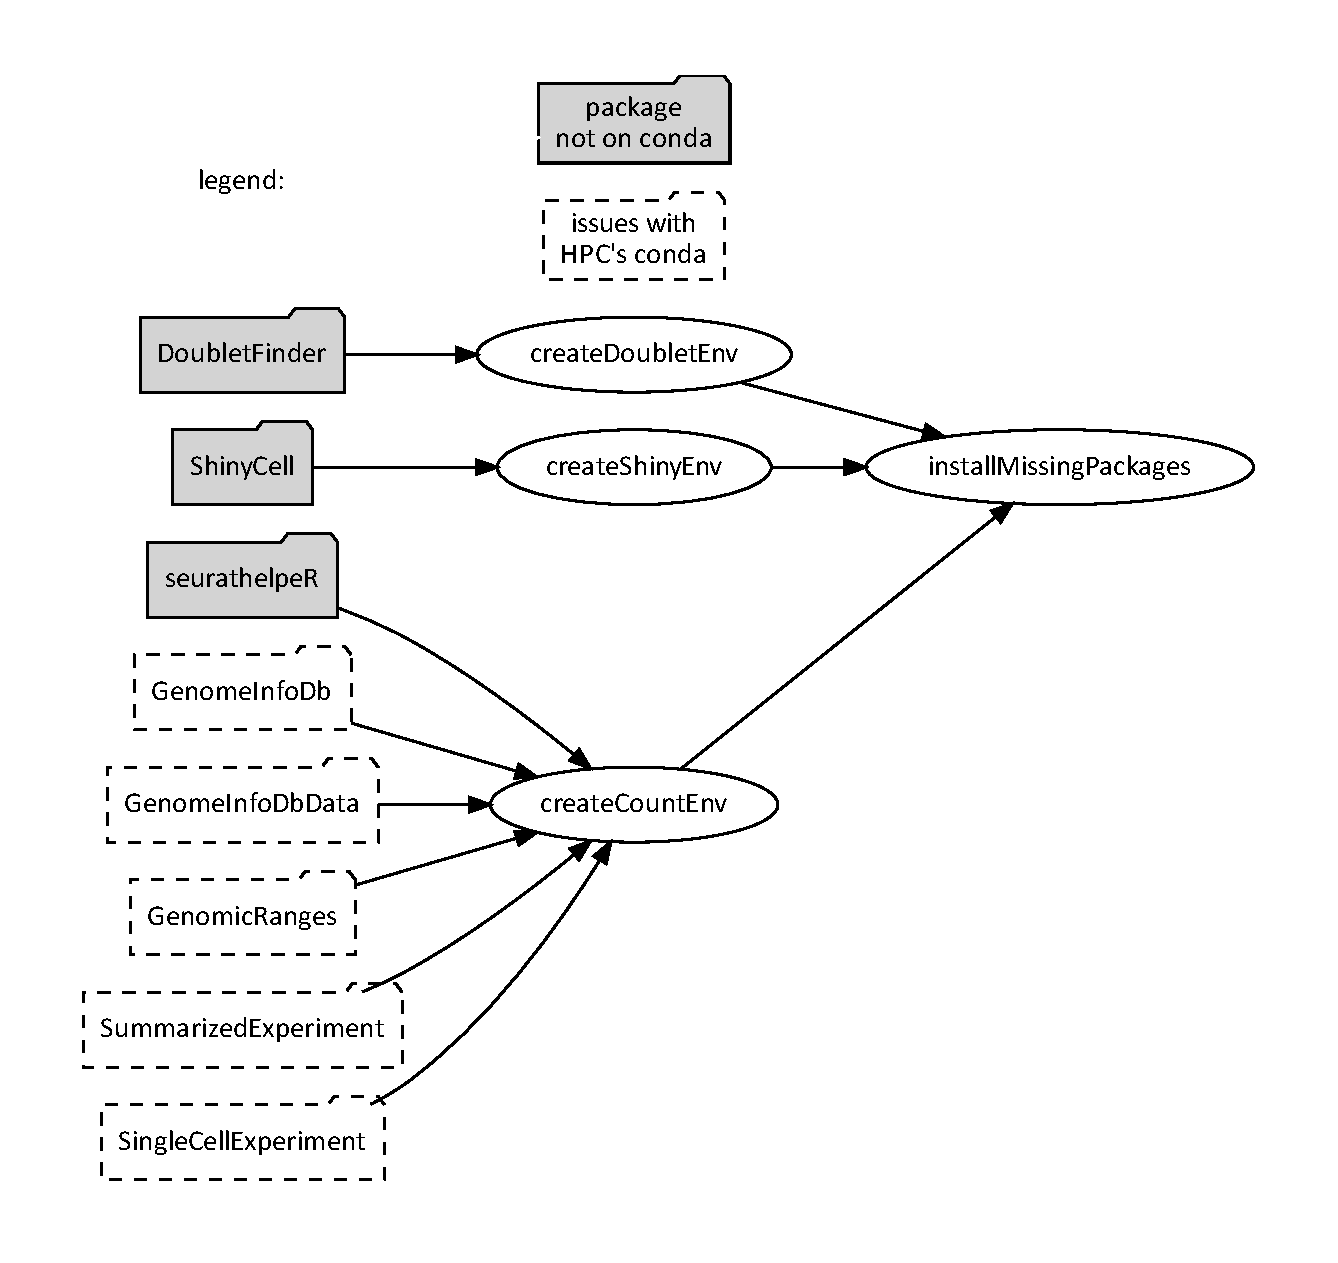
\includegraphics[width=1\textwidth]{figures/installRun.pdf}}
	\caption{How the installation run works.}
	\label{fig:installRun}
\end{figure}
 
\begin{figure}[h!]
	%\includesvg[width=\textwidth]{figures/pipelineRun.pdf}
	\centering
	\makebox[\textwidth][c]{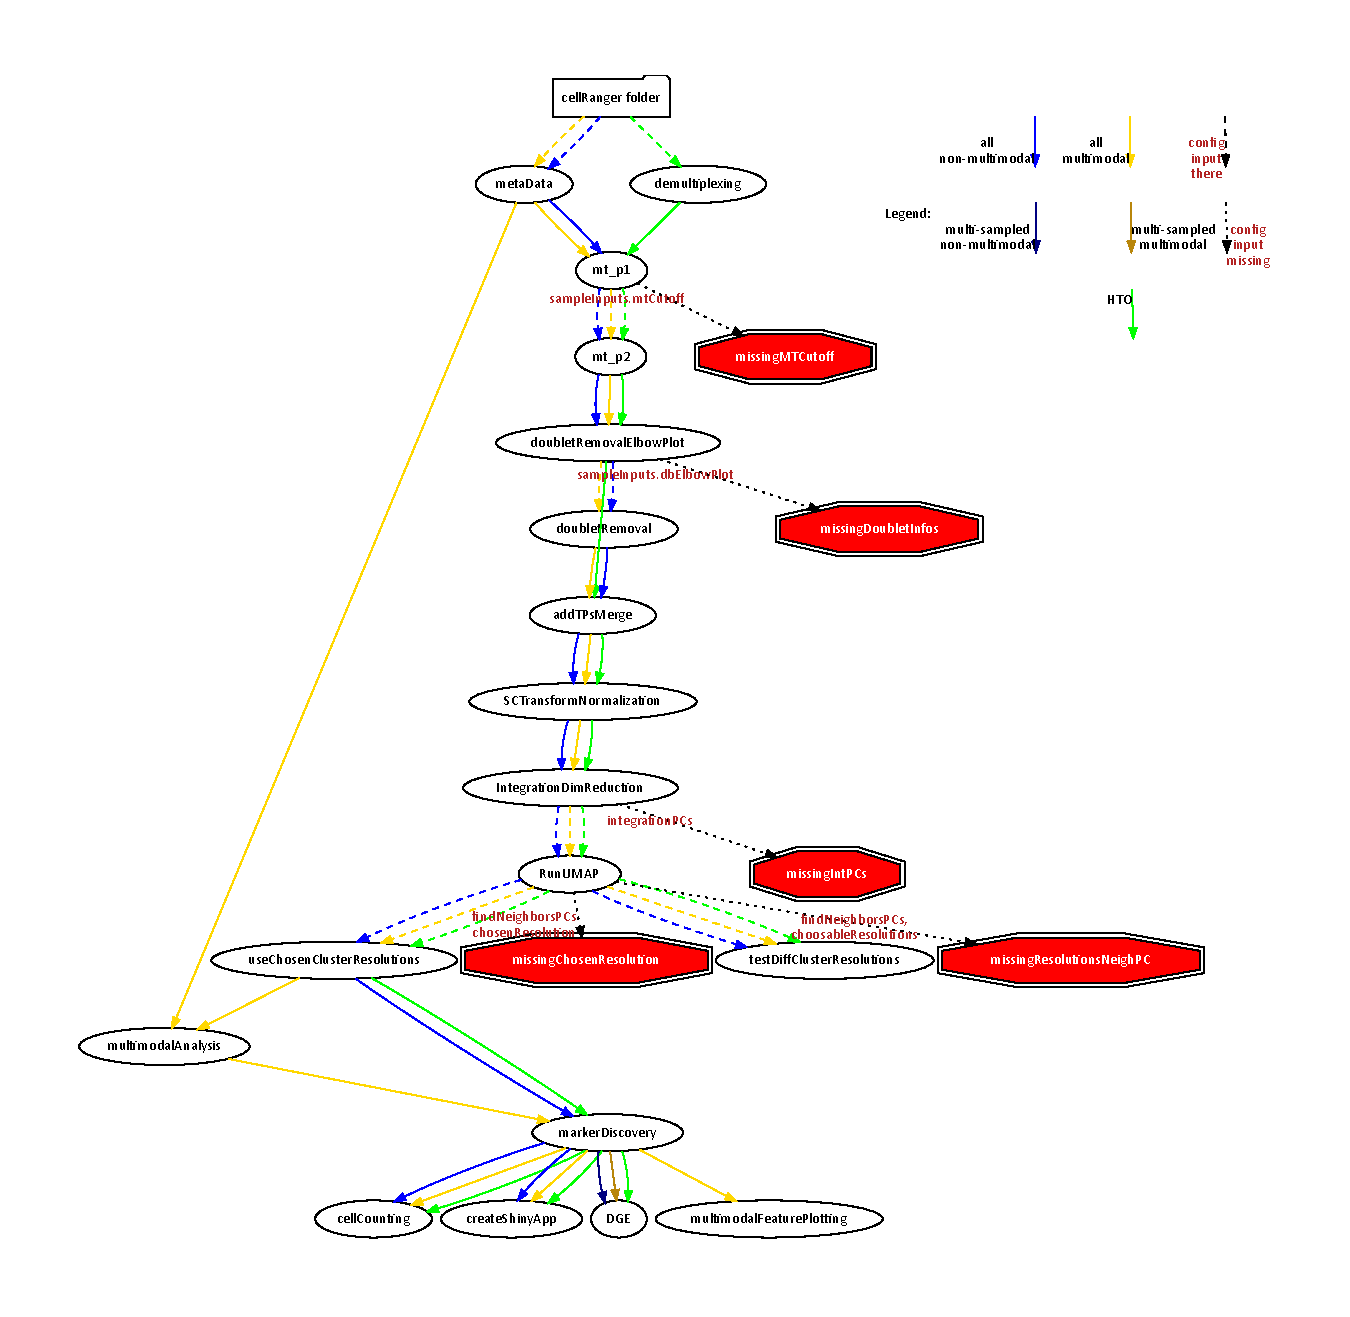
\includegraphics[width=1.55\textwidth]{figures/pipelineRun.pdf}}
	\caption{The three workflow ways.}
	\label{fig:pipelineRun}
\end{figure}

\subsection{metaData}
The metaData step is used for both non-multimodal and multimodal datasets though not for HTO. It reads the 10X Cellranger folder and transforms the dataset into a SeuratObject. It will then add the sample names to each sample and create an output for each sample respectively called \textbf{sample\_name}.metaData.rds. If the dataset had additional data like protein data it will create an additional output called \textbf{projectname}.rawData.rds.

\subsection{demultiplexing}
The demultiplexing step is for HTO datasets. Here too, the 10X Cellranger folder is read and transformed into a SeuratObject. The HTO data is added as an assay and the SeuratObject is demultiplexed. A scatter plot called \textbf{projectname}.HTOscatter.pdf. is created and then the doublets are removed. The sample name is then added to each sample and each sample is outputted as \textbf{sample\_name}.demux.rds.

\subsection{mt\_p1}
This step calculates the percentage of counts belonging to mitochondrial reads for each cell. It will then create violin plots called \textbf{sample\_name}.mt.before.pdf from which the user should determine at what percentage of mitochondrial reads the cells of a sample should be filtered. After this step a \textbf{\textit{MissingInputError}} will be thrown until the user enters a percentage for each sample into the "mtCutoff" slot in the config.yaml.

\subsection{mt\_p2}
After the percentages where entered into the config.yaml, this step will remove all cells that had a percentage of mitochondiral reads greater than the cutoff value. It will then create a \textbf{sample\_name}.mt.after.pdf plot for each sample for a before and after comparison.

\subsection{doubletRemovalElbowPlot}
For each sample this step performs SCT normalization and PCA before creating an elbow plot. The elbow plot is used to determine the "dbElbowPlot" in the config.yaml. The value describes the PCs/dimensions for the doublet removal. A \textbf{\textit{MissingInputError}} will be thrown until an value is entered for each sample.

\subsection{DoubletRemoval}
Only if not HTO, otherwise this step is skipped. Here DoubletFinder removes the doublets.

\subsection{addTPsMerge}
Here additional meta data from "otherMetaName" and "otherMetaData" is added to the respective samples as well as all possible combinations created from the two configs. E.g., if the dataset has condition and timepoint as meta data the combination condition.timepoint will be created. Afterwards all samples are combined into a single dataset again and outputted as \textbf{projectname}.preprocessedO.rds.

\subsection{SCTransformNormalization}
SCT normalization is performed for each sample in the dataset.

\subsection{IntegrationDimReduction}
If the dataset has multiple samples, Seurat's integration via anchors is performed followed by PCA. Otherwise only PCA is performed. Then the elbow plot \textbf{projectname}.integratedElbowPlot.pdf is created, so the user can choose the number of PCs for UMAP. A \textbf{\textit{MissingInputError}} will be thrown until the number of PCs us entered as "integrationPCs" in the config.

\subsection{RunUMAP}
UMAP with the number of PCs of "integrationPCs" from config is performed. The two plots \textbf{projectname}.umappedDimPlot.pdf and \textbf{projectname}.umappedElbowPlot.pdf are created. The elbow plot is used to find the number of PCs for "findNeighborsPCs" in config which describes the number of PCs used in Seurat's "FindNeighbors" function. Until a value is entered into the config, the \textbf{\textit{MissingInputError}} will be thrown. The error will also be thrown until "choosableResolutions" is filled out. More on that in the next subsection.

\subsection{testDiffClusterResolutions \& useChosenClusterResolution}
Next, clustering should be performed. Seurat controls the number of clusters with a "resolution" variable in the FindClusters function. A resolution below 1 gives less while a resolution above 1 gives more clusters. The step testDiffClusterResolutions is used to create multiple plots with different resolutions from "choosableResolutions" from the config if the user does not know what resolution is used. After choosing a resolution useChosenClusterResolution is perfomed for the actual clustering of the dataset using "chosenResolution" in the dataset.

\subsection{multimodalAnalysis}
This is only performed if the dataset is multimodal. Here, the additional data like protein data will be added to the dataset. However, currently only "Antibody Capture" can be added.

\subsection{markerDiscovery}
The dataset is normalized and scaled. Gene markers are found through the FindAllMarkers function of Seurat. These markers are written into two .CSV files in csv/.\\ \textbf{projectname}.compareGE\_inAll.markers.csv contains the output of FindAllMarkers while \textbf{projectname}.compareGE\_inAll.avgExpression.csv contains the output of AverageExpression.

\subsection{cellCounting}
For each condition or condition combination a bar plot is created containing the relative number of cells in a cluster grouped by condition type. If there are multiple samples error bars will be created describing the standard deviation.

\subsection{createShinyApp}
A shiny app for the dataset is created through ShinyCell.

\subsection{DGE}
For each condition (combination) differentially expressed genes are calculated by comparing each condition type in each cluster with each other and saved in .CSV files. If one condition has less than three cells compared to the other condition the comparison is skipped and noted in finishedDGE.txt. Only for multi-sampled dataset.

\subsection{multimodalFeaturePlotting}
For each feature in the extra assay a feature plot \textbf{feature}.adtFeatureProtein.pdf is created.